\subsection{Design du système}
    Le système se dècoupe essentiellement en 3 parties:
    \begin{itemize}
        \item[-] Coté utilisateur
        \item[-] Coté jeu
        \item[-] Coté Server   
    \end{itemize}
    \subsubsection{Coté utilisateur}
        % \makebox[\textwidth]{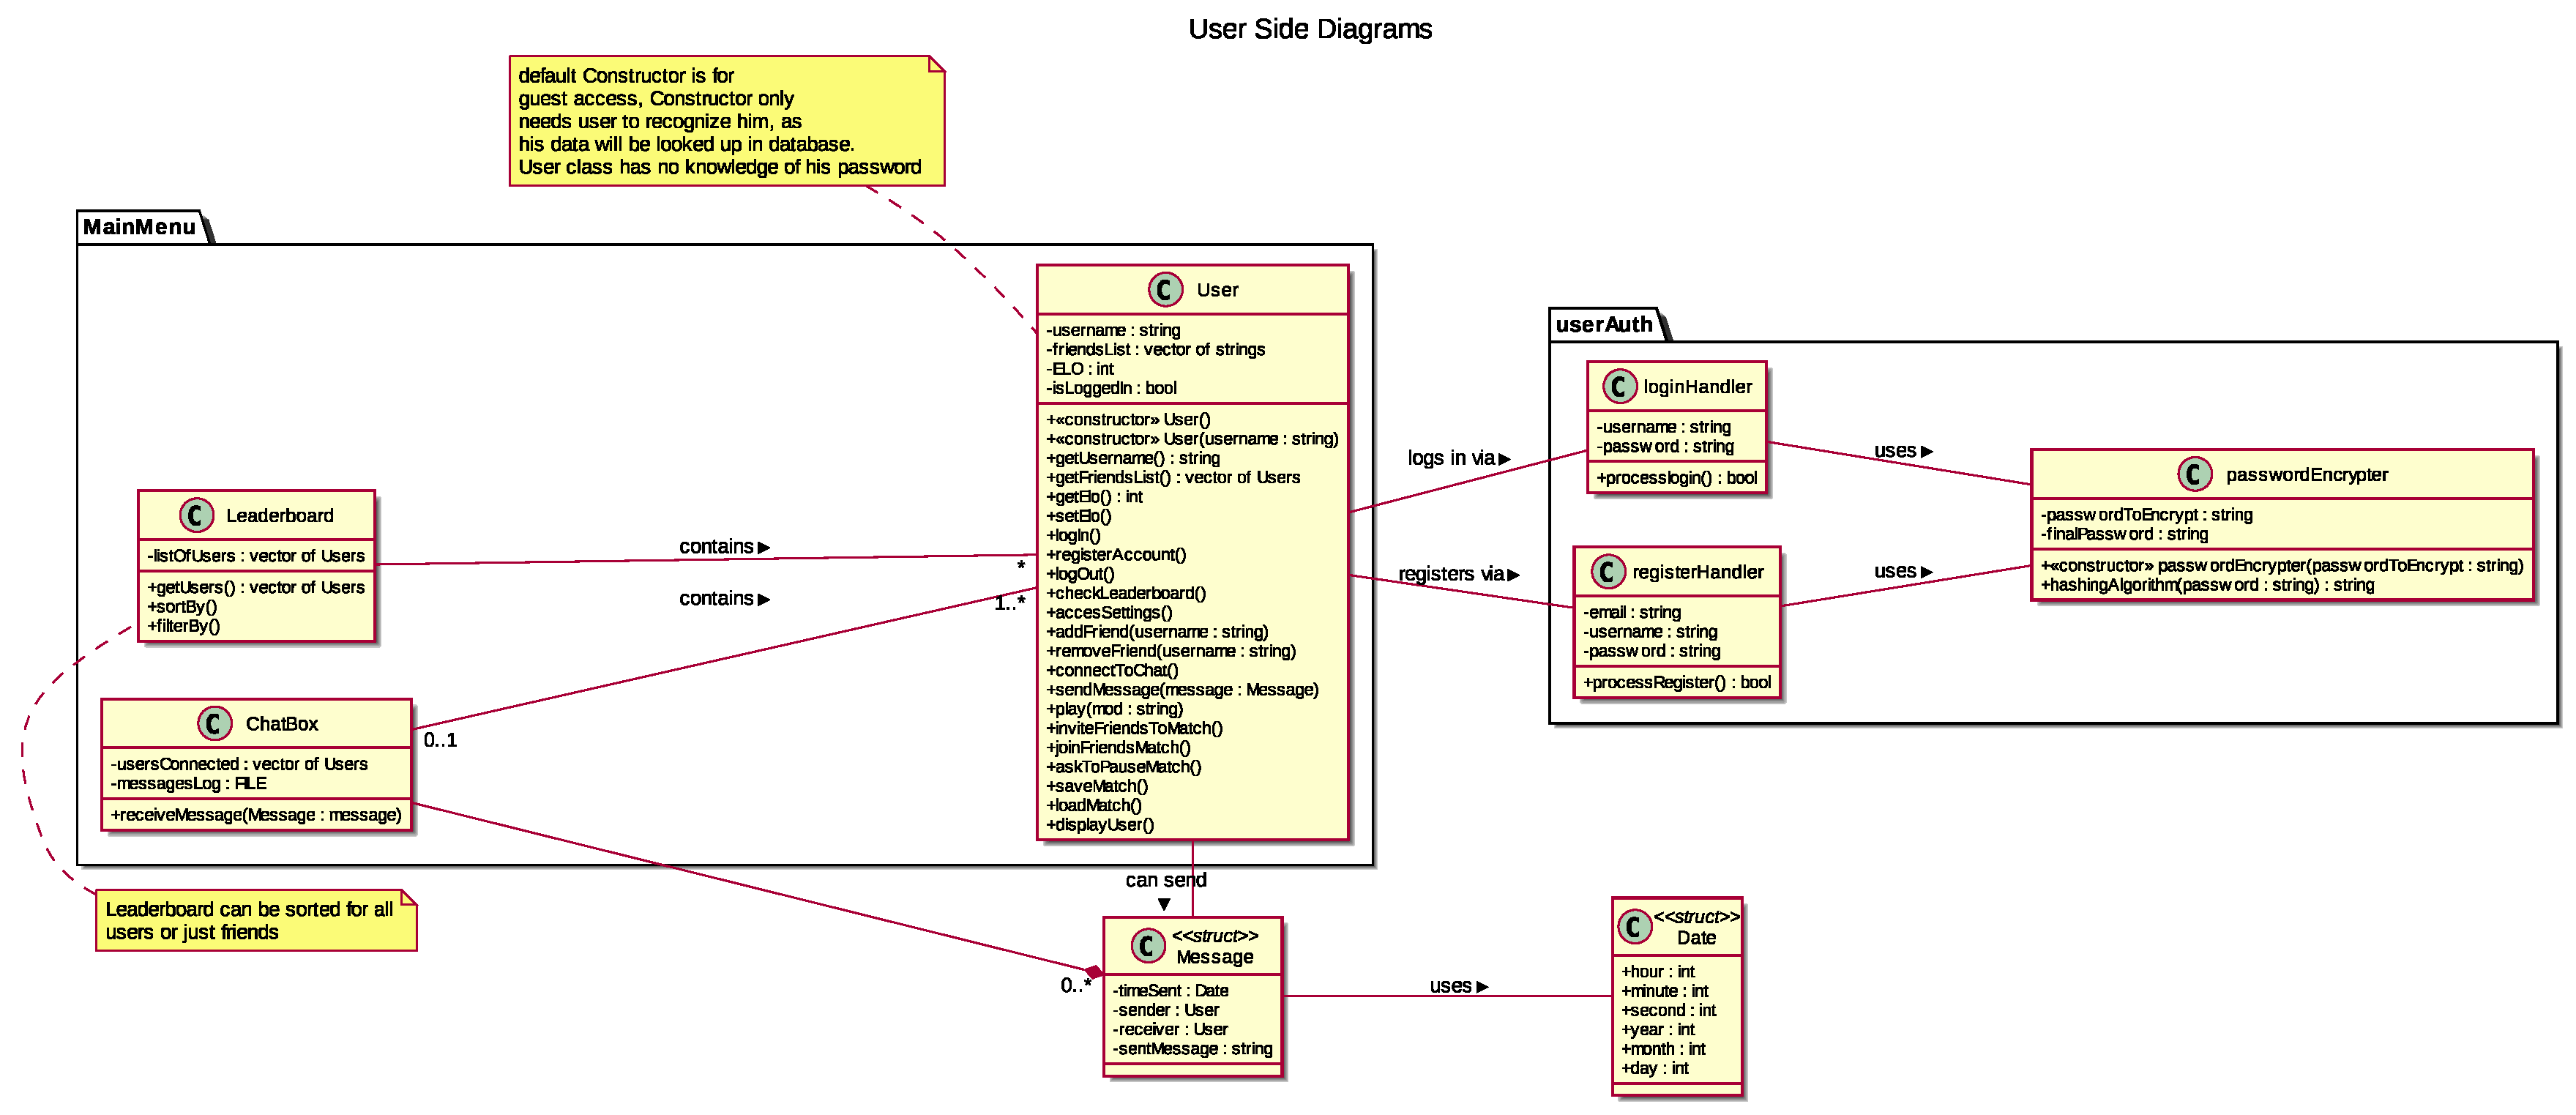
\includegraphics[width=\textwidth]{UserSideDiagrams.eps}}
    \addimg{img/6_UserSideDiagrams.eps}{width=\textwidth}{Diagrammes du côté utilisateur}{usrside}
        L'utilisateur entre dans le jeu comme une sorte de "Guest",
        ne pouvant pas utiliser l'interface
        Pour pouvoir utiliser les fonctionnalités de Quoridor, l'utilisateur doit se connecter
        à son compte ou en créer un s'il n'en a pas. Les deux evenements passeront à travers des "handlers", qui
        géreront les requetes en passant à travers un database et le Server. Après s'etre connecté.e, l'utilisateur aura accès à toutes les fonctionnalités
        que offre le logiciel (cfr. Sections 2 et 4).
    \subsubsection{Coté jeu}
        % \makebox[\textwidth]{\includegraphics[width=\textwidth]{GameDiagrams.eps}} 
    \addimg{img/6_GameDiagrams.eps}{width=\textwidth}{Diagrammes de jeu}{gameside}
    

